\documentclass{article}
\usepackage{amsmath,amssymb,amsthm}
\usepackage{enumerate}
\usepackage{mathtools}
\usepackage{graphicx}
\usepackage{caption}
\newtheorem{theorem}{Theorem}
\newtheorem{question}[theorem]{Question}
\newtheorem{answer}[theorem]{Solution}
\begin{document}
\begin{question}
	Show that the vectors $\begin{pmatrix} 
		 +2\\-1\\+1 
	\end{pmatrix}$, $\begin{pmatrix} 
	 +1\\-3\\-5 
\end{pmatrix}$ and $\begin{pmatrix} 
+3\\-4\\-4 
\end{pmatrix}$ form the vertices of a right angled triangle.
\end{question}
Solution. Let $v1$, $v2$ and $v3$ be given vectors such that $v1 =\begin{pmatrix} 
	+2\\-1\\+1 
\end{pmatrix}$,\\     
$v2= \begin{pmatrix} 
+1\\-3\\-5 
\end{pmatrix}$ and $v3= \begin{pmatrix} 
+3\\-4\\-4 
\end{pmatrix}$.\\
To show that $v1$, $v2$ and $v3$ form the vertices of a right anled triangle. First we need to show that $v1$, $v2$ and $v3$ are indeed vertices of a triangle.\\
For this we need to see if the vertices satisfy trianle inequality. Let $a$, $b$ and $c$ denote the length of vertices $v1-v2$, $v2-v3$ and $v3-v1$. Now,\\
$a=\sqrt{41}$, $b=\sqrt{6}$ and $c=\sqrt{35}$. We can see that  $a+b>c$, 
$a+c>b$ and $b+c >a$. Thus, the given vertices $v1$, $v2$ and $v3$ form the vertices of a triangle. Let vertices $v1$, $v2$ and $v3$ be represented as A, B and C respectively.\\


 \begin{figure}[!htb]
	\center{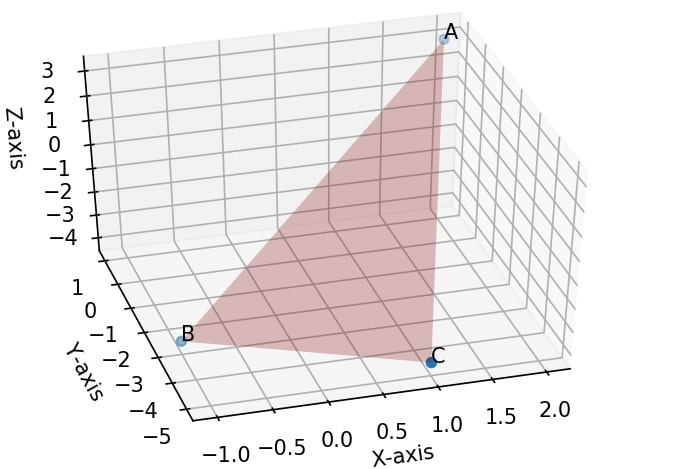
\includegraphics[width=\textwidth]
		{assignment1fig-1.jpg}}
	\caption{\label{fig1}}
\end{figure}

Also triangle formed by A,B and C is ploted in Figure 1, as seen $\triangle ABC$ is right angled at C. This is because $<A-C, B-C>$ which is equal to $(A-C)^T(B-C) $ is indeed $=0$. This means (A-C)$\perp$(B-C). Thus, proving that $\triangle$ABC is right angled triangle at C.


\end{document}
